\documentclass[border=10pt]{standalone}

\usepackage{tikz}
\usepackage{tikzsymbols}
\usetikzlibrary{calc,patterns,shapes.geometric}

\def\centerarc[#1](#2)(#3:#4:#5){\draw[#1] ($(#2)+({#5*cos(#3)},{#5*sin(#3)})$) arc (#3:#4:#5);}

\begin{document}
	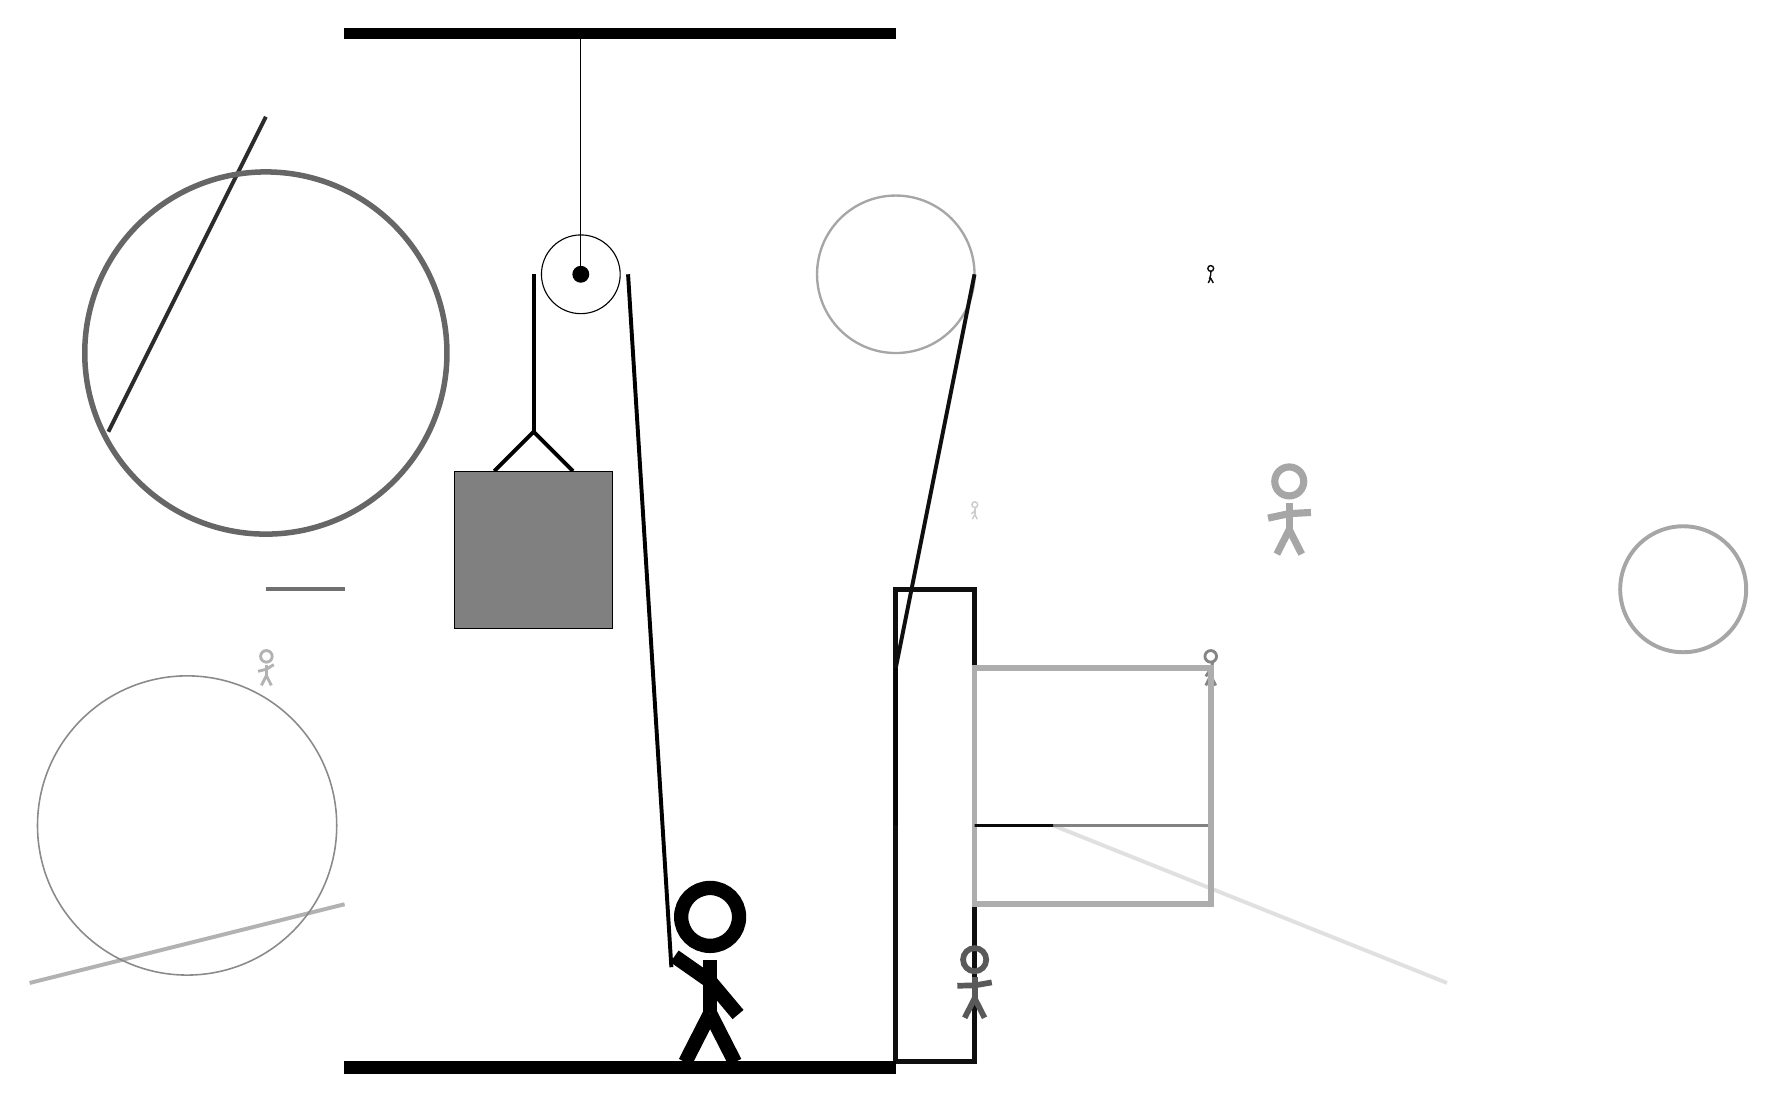
\begin{tikzpicture}
		%%%%% START %%%%%
		
		\draw[fill=black] (-2, 10) rectangle (5, 10.125);
		
		\draw[line width=0.6mm, color=black!94] (5, 3) rectangle (6, -3);
		
		\draw[line width=0.5mm, color=black!12](7, 0) -- (12, -2);
		\draw [line width=0.3mm, color=black!35](5, 7) circle (1.0);
		\draw[line width=0.5mm, color=black!83](-3, 9) -- (-5, 5);
		\node[line width=0.2mm, color=black!35] at (10, 4) {\Strichmaxerl[5][12][3]};
		\draw [line width=0.7mm, color=black!60](-3, 6) circle (2.3);
		
		\draw[line width=0.5mm, color=black!30](-2, -1) -- (-6, -2);
		
		\draw[line width=0.5mm, color=black!49] (7, 0) rectangle (9, 0);
		\draw [line width=0.5mm, color=black!35](15, 3) circle (0.8);
		
		\node[line width=0.2mm, color=black!95] at (9, 7) {\Strichmaxerl[1][73][89]};
		\node[line width=0.5mm, color=black!30] at (-3, 2) {\Strichmaxerl[2][14][32]};
		\draw [line width=0.2mm, color=black!46](-4, 0) circle (1.9);
		\draw[line width=0.5mm, color=black!94](5, 2) -- (6, 7);
		\node[line width=0.3mm, color=black!48] at (9, 2) {\Strichmaxerl[2][55][73]};
		\draw[line width=0.7mm, color=black!32] (6, 2) rectangle (9, -1);
		\draw[line width=0.3mm, color=black!96] (6, 0) rectangle (7, 0);
		
		\draw[line width=0.5mm, color=black!56](-3, 3) -- (-2, 3);
		
		\node[line width=0.2mm, color=black!20] at (6, 4) {\Strichmaxerl[1][37][76]};
		\draw[line width=0.5mm, color=black!98] (5, 0) rectangle (5, 2);
		
		\node[line width=0.6mm, color=black!65] at (6, -2) {\Strichmaxerl[4][1][10]};
		
		\draw (1, 7) circle (0.5);
		\draw[fill=black] (1, 7) circle (0.1);
		\draw (1, 10) -- (1, 7);
		
		\draw[line width=0.5mm] (-0.1, 4.5) -- (0.4, 5.0) -- (0.9, 4.5);
		\draw[fill=black!50] (-0.6, 4.5) rectangle (1.4, 2.5);
		
		\draw[line width=0.5mm] (0.4, 7) -- (0.4, 5.0);
		\centerarc[line width=0.5mm](1, 7)(0:180:0.6);
		\draw[line width=0.5mm](1.6, 7) -- (2.15, -1.8);
		
		\node at (2.6, -1.9) {\Strichmaxerl[10][-35][-50]};
		
		\draw[fill=black] (-2, -3) rectangle (5, -3.15);
		
		%%%%% END %%%%%
	\end{tikzpicture}
\end{document}